
\section{\lsystem processing library}
\label{sec:design-library}

The main design goal of the \lsystem processing library was that it should be simple to extend.
It should be possible to alter the processing of an \lsystem without needing to change the whole processing system.
This behavior is achieved by its modular design -- input is processed within a set of connected components.
Each component is specialized for one particular activity: for example, symbol rewriting or the rendering of an image.
Both components and connections are definable by the user.

A component-based modular system has many advantages over a monolithic system.
Probably the biggest advantage, one already discussed, is its ease of extensibility.
It is simple to implement the extension of a component and include it into the system.
It is also possible to improve existing components and extend system capabilities.
A simple illustration of how this component system extension works is shown in \autoref{fig:extensionExample}.
The first system (Fig. \ref{fig:extensionExampleBase}) was extended by a gravity simulation component being added to give the second system (Fig. \ref{fig:extensionExampleExtended}).
The possible results are shown in \autoref{fig:extensionExampleResult}.

Another advantage lies the in specialization of its components.
Specialized components are easier to implement and the outcome will most likely have less bugs.
Specialization also helps to make a system more robust because individual components can be tested separately.
Tests for a single component are easier to write and they can test situations which cannot be tested for on the whole system.

\begin{figure}[h]
	\centering
	\subfloat[Simple component-based system]{
		\begin{tikzpicture}[->,auto,>=latex,shorten >=2pt]
			\node (in) [coord] {};
			\node (rw) [block, right of=in, node distance=3cm] {Rewriter};
			\node (int) [block, right of=rw, node distance=4cm] {Interpreter};
			\node (out) [coord, right of=int, node distance=3cm] {};
			
			\draw (in) -- node {input} (rw);
			\draw (rw) -- (int);
			\draw (int) -- node {output} (out);
		\end{tikzpicture}
		\label{fig:extensionExampleBase}
	}
	\\
	\subfloat[Extended component-based system]{
		\begin{tikzpicture}[->,auto,node distance=4cm,>=latex,shorten >=2pt]
			\node (in) [coord] {};
			\node (rw) [block, right of=in, node distance=3cm] {Rewriter};
			\node (g) [blockx, right of=rw] {Gravity simulation};
			\node (int) [block, right of=g] {Interpreter};
			\node (out) [coord, right of=int, node distance=3cm] {};
			
			\draw (in) -- node {input} (rw);
			\draw (rw) -- (g);
			\draw (g) -- (int);
			\draw (int) -- node {output} (out);
		\end{tikzpicture}
		\label{fig:extensionExampleExtended}
	}
	\caption{The extension of component-based processing system}
	\label{fig:extensionExample}
\end{figure}

\begin{figure}[h]
	\centering
	\subfloat[Original tree model (no effect of gravity)]{
		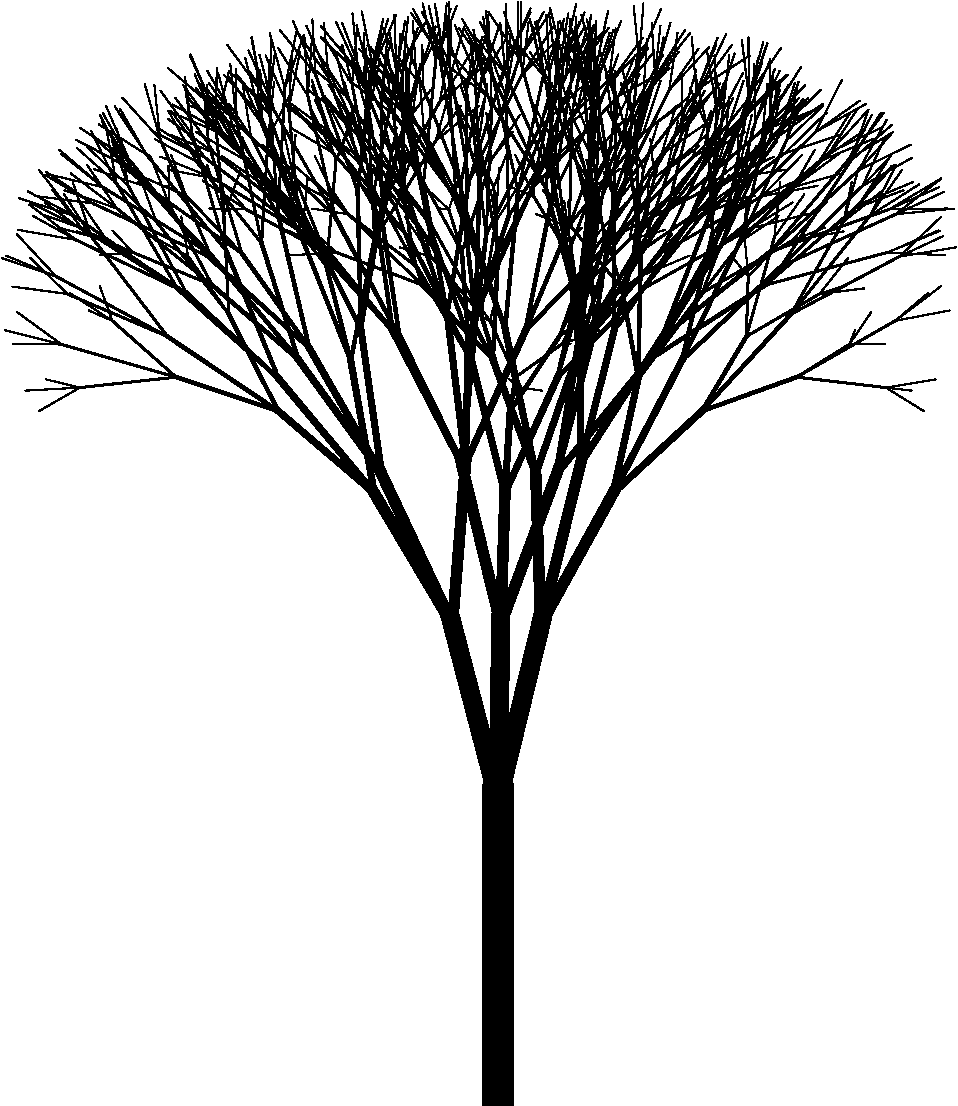
\includegraphics[scale=0.4]{ComponentSystemGravityOff}
	} ~
	\subfloat[Tree model with simulated gravity]{
		
\includegraphics[scale=0.4]{ComponentSystemGravityOn}
	}
	\caption{Possible outputs from process systems in \autoref{fig:extensionExample}}
	\label{fig:extensionExampleResult}
\end{figure}



\subsection{Input form}

Input is an important part of an application.
\lsystems have no standardized input: for example, like programming languages.
Every implementation of an \lsystem processor uses its own variant of the input.

The main goals for input design are simplicity and universality.
With simple input there is lower threshold for a new user to start using an application.
Complicated input might well discourage many potential users.
Universal input means that \textit{everything} is possible to define by input, including definitions of \lsystems, configuration of components, etc.

Generally there are two basic types of input, the graphic interface and source code.
Source code was chosen to be he input because it is better for saving, sharing and versioning.
Statements can be easily commented upon, thus the ideas behind the code can be saved with it.
Parts of the code can be copy-pasted and the syntax can be extended.
Parsing of source code is quite complex but the input interface can be just one text area.

To achieve good readability of input source code the syntax will have to be rich in keywords.
This should ensure that even new users will understand the statements.
With source code input it is still possible to create a second type of input -- the graphic interface.
This can be achieved by source code designers but this will be left to a future extension.


\subsection{Input syntax}

Everything can be described by input.
By everything is meant \lsystem definitions, configuration of components, definitions of component systems, which \lsystem to process with which component system etc.
This is important for easy saving and sharing.

The following list describes concrete entities which are possible to describe with source code.

\begin{itemize*}
	\item Global constant
	\item Global function
	\item \lsystem definition
		\begin{itemize*}
			\item Local constant
			\item Local function
			\item Component property assignment
			\item Component symbol property assignment
			\item Symbol interpretation -- defined interpretation for one or more \lsystem symbols
			\item Rewrite rule
		\end{itemize*}
	\item Process configuration -- definition of component system
		\begin{itemize*}
			\item Component
			\item Container -- components in container a can be reassigned when an \lsystem is processed by process configuration
			\item Connection -- defines the connection between two components
		\end{itemize*}
	\item Process statement -- defines processing of the \lsystem with process configuration
		\begin{itemize*}
			\item Container component reassign -- change of component in container
			\item Additional \lsystem statements -- additional \lsystem statements which can alter the processed \lsystem
		\end{itemize*}
\end{itemize*}

A full reference of the input syntax is given in appendix \ref{chap:syntax}.
A small example of input source code together with the result is shown in \autoref{fig:scExample}.

\newsavebox{\lstBoxParams}
\begin{lrbox}{\lstBoxParams}
\begin{Lsystem50}
lsystem SierpinskiGasket {
	set symbols axiom = + R;
	set iterations = 7;

	interpret L R as DrawForward(
		2 ^ -currentIteration
		* 700);
	interpret + as TurnLeft(60);
	interpret - as TurnLeft(-60);

	rewrite L to R + L + R;
	rewrite R to L - R - L;
}
process all with SvgRenderer;
\end{Lsystem50}
\end{lrbox}

\begin{figure}[h!]
	\subfloat{
		\usebox{\lstBoxParams}
	} \hfill
	\subfloat{
		\minipage{0.47\linewidth}\noindent
		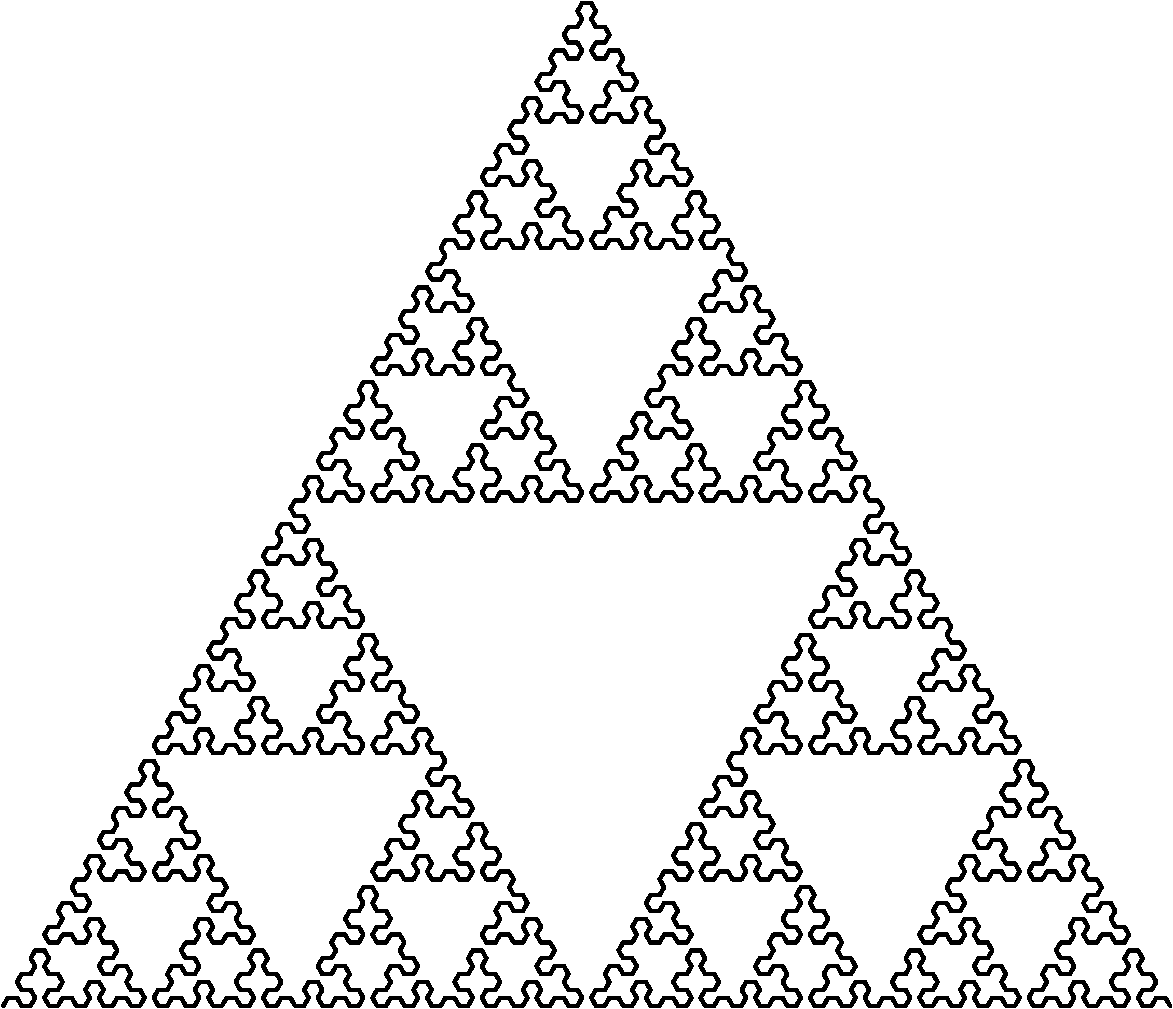
\includegraphics[width=\textwidth]{SierpinskiGasket}
		\endminipage
	}
	\caption{Example of source code along with the result -- Sierpinski gasket}
	\label{fig:scExample}
\end{figure}


\subsubsection{Value types}

The \lsystem processing library allows to use two types of values for constants or for configuration of components.
The first type is a \emph{number} and it is stored as floating point value with about 15 significant digits.
The numbers can be specified in 5 formats:

\begin{itemize*}
	\item floating-point format like 24, -8.1, 2e-10, 3141.59e3,
	\item binary format with prefix \emph{0b} like 0b100101 or 0b0111011,
	\item octal format with prefix \emph{0o} like 0o54607, 0o776,
	\item hexadecimal format with prefix \emph{0x} like 0xFFBF00, 0x13a4F,
	\item hexadecimal format with prefix \# like \#332211 (this is handy for colors).
\end{itemize*}

The second type is a \emph{array}.
The elements in the array can be both the constants and the arrays.
The array is started and ended by a brace and the values are separated by a comma.
The syntax of the array is illustrated in \autoref{lsys:arrays}.

\begin{Lsystem}[label=lsys:arrays,caption={Example of array syntax.}]
let const = 0xAF + 1.2e1;
let array = {1, 2, {3.1, 3.2, 3.3}, const, 5, {}};
\end{Lsystem}


\subsubsection{\lsystem inheritance}

The \lsystem can \emph{inherit} (extend) all features from some other L-system.
This feature should minimize code repetition and allows to define base \lsystems in the standard library to simplify the work with \lsystems (see appendix \ref{sec:stdLibLsystems}).

The pre-existing L-system is called \emph{base} or \emph{ancestor} and the new L-system is called \emph{derived} L-system or \emph{child} L-system.
Inheritance L-system statements follows a simple rule: the derived L-system will redefine definitions of the base L-system.
The result of \autoref{lsys:inherit} is \texttt{B B B B B A} (the first process statement) and \texttt{X X A} (the second process statement).

\begin{Lsystem}[label=lsys:inherit,caption={Example \lsystems inheritance.}]
lsystem BaseLsystem {
	set symbols axiom = A;
	set iterations = 5;
	rewrite A to B A;
}
lsystem DerivedLsystem extends BaseLsystem {
	set iterations = 2;
	rewrite A to X A;
}
process BaseLsystem with SymbolPrinter;
process DerivedLsystem with SymbolPrinter;
\end{Lsystem}

It is possible to inherit more than one L-system.
Their statements are redefined in the same order as stated in the definition.
The result of \autoref{lsys:inheritMore} is \texttt{Y Y A} (the first process statement) and \texttt{X X A} (the second process statement).

\begin{Lsystem}[label=lsys:inheritMore,caption={Example of the array syntax.}]
lsystem BaseLsystemX {
	set symbols axiom = A;
	set iterations = 5;
	rewrite A to X A;
}
lsystem BaseLsystemY {
	rewrite A to Y A;
}
lsystem DerivedLsystemXY extends BaseLsystemX, BaseLsystemY {
	set iterations = 2;
}
lsystem DerivedLsystemYX extends BaseLsystemY, BaseLsystemX {
	set iterations = 2;
}
process DerivedLsystemXY with SymbolPrinter;
process DerivedLsystemYX with SymbolPrinter;
\end{Lsystem}


\subsection{Source code compilation}
\nomenclature{AST}{abstract syntax tree}

Source code compilation has two steps as shown in \autoref{fig:compilePipeline}.
The first step is parsing the of source code to the \emph{abstract syntax tree} (henceforth called AST).
The syntax parser is generated by the \emph{FsYacc} parser generator which will guarantee a robust and extensible syntax paring (for details see \autoref{sec:parsingImplementaion}).
Each node of the AST will contain information about its position in the original source code.
At this point the AST can be used for syntax highlighting or source code formatting.

\begin{figure}[h]
	\centering
	\begin{tikzpicture}[->,auto,node distance=4cm,>=latex,shorten >=2pt]
		\node (in) [coord] {};
		\node (yacc) [block, right of=in] {Lexer \& parser};
		\node (comp) [block, right of=yacc] {Compiler};
		\node (out) [coord, right of=comp] {};
		
		\draw (in) -- node {source code} (yacc);
		\draw (yacc) -- node {AST} (comp);
		\draw (comp) -- node {semantic tree} (out);
	\end{tikzpicture}
	\caption{Source code compilation system}
	\label{fig:compilePipeline}
\end{figure}

The abstract syntax tree (AST) for \autoref{lsys:ast} is shown in \autoref{fig:ast}.
You can see that expressions are not parsed as a tree, they are placed in a linear list under the \emph{Expression} node.
This is because operators (and their precedences) can be defined by the user, thus parser can not parse expressions where operator precedence is needed (like $2 + 3 * 4$).
Expressions will be parsed to the expression tree by the compiler in the next step.

\begin{Lsystem}[label=lsys:ast,caption={Constant definition statement for example of AST}]
let angle = 90 + 5 * random();
\end{Lsystem}

\tikzstyle{ast} = [draw, fill=blue!12, rectangle split, rectangle split parts=2, minimum height=2em]
\tikzstyle{astx} = [draw, fill=red!12, rectangle, rounded corners=1mm]

\begin{figure}[p]
	\centering
	\begin{tikzpicture}[child anchor=north,>=latex] %level/.style={sibling distance=33mm/#1},
		\node [ast] {Constant definition \nodepart{second} \footnotesize ln: 1, col: 1--30}
			[level distance=25mm, sibling distance=30mm]
			child { node [astx] {let} }
			child { node [ast] {Identificator \nodepart{second} \footnotesize ln: 1, col: 5--9}
				[level distance=14mm] child { node [astx] {angle} }
			}
			child { node [astx] {=} }
			child { node [ast] {Expression \nodepart{second} \footnotesize ln: 1, col: 13--29}
				[level distance=40mm]
				child { node [ast] {Number \nodepart{second} \footnotesize ln: 1, col: 13-14} child[level distance=14mm] { node [astx] {90} } }
				child { node [ast] {Operator \nodepart{second} \footnotesize ln: 1, col: 16} child[level distance=14mm] { node [astx] {+} } }
				child { node [ast] {Number \nodepart{second} \footnotesize ln: 1, col: 18} child[level distance=14mm] { node [astx] {5} } }
				child { node [ast] {Operator \nodepart{second} \footnotesize ln: 1, col: 20} child[level distance=14mm] { node [astx] {*} } }
				child { node [ast] {Function \nodepart{second} \footnotesize ln: 1, col: 22--29} child[level distance=14mm] { node [astx] {random} } }
				child [missing] {}
				child [missing] {}
			}
			child { node [astx] {;} }
			;
	\end{tikzpicture}
	\caption{Abstract syntax tree parsed from \autoref{lsys:ast}}
	\label{fig:ast}
\end{figure}

The next step of source code processing is compilation of the AST into the \emph{semantic tree} (henceforth called ST). \nomenclature{ST}{semantic tree}
Unlike the AST the semantic tree contains only data (no keywords or metadata about position).
However the nodes of the semantic tree have a reference to the corresponding AST nodes to make it possible to get the metadata, for example, for reporting the locations of compilation errors.
The semantic tree in \autoref{fig:st} is created by compiling the AST in \autoref{fig:ast}.
A more complex semantic tree obtained from \autoref{lsys:stComplex} is shown in \autoref{fig:stComplex}.

\tikzstyle{st} = [draw, fill=blue!12, rectangle split, rectangle split parts=2, minimum height=2em]
\tikzstyle{stx} = [draw, fill=blue!12, rectangle, minimum height=2em]

\begin{figure}[p]
	\centering
	\begin{tikzpicture}[child anchor=north,>=latex] %level/.style={sibling distance=33mm/#1},
		\node [st] {Constant definition \nodepart{second} \footnotesize name: angle}
			[level distance=18mm, sibling distance=30mm]
			child { node [st] {Operator \nodepart{second} \footnotesize addition} 
				child { node [st] {Number \nodepart{second} \footnotesize 90} }
				child { node [st] {Operator \nodepart{second} \footnotesize multiplication} 
					child { node [st] {Number \nodepart{second} \footnotesize 5} }
					child { node [st] {Function \nodepart{second} \footnotesize random} }
				}
			}
			;
	\end{tikzpicture}
	\caption{Semantic tree created by compilation of the AST in \autoref{fig:ast}}
	\label{fig:st}
\end{figure}


\begin{Lsystem}[label=lsys:stComplex,caption={This source code results in the semantic tree shown in \autoref{fig:stComplex}}]
let iterBase = 2;
lsystem Octahedron {
	set symbols axiom = F;
	set iterations = iterBase + 1;
	interpret F as DrawForward(100, 2);
	interpret + as TurnLeft(45);
	rewrite F to F + F;
}
process all with SvgRenderer;
\end{Lsystem}

\begin{figure}[p]
	\centering
	\begin{tikzpicture}[grow'=right,child anchor=west,>=latex]
		\node [stx] {Input}
			[level distance=25mm, sibling distance=15mm]
			child { node [st] {Constant definition \nodepart{second} \footnotesize name: iterBase}
				[level distance=35mm]
				child {	node [st] {Number \nodepart{second} 2} }
			}
			child [missing] {}
			child [missing] {}
			child [missing] {}
			child [missing] {}
			child { node [st] {L-system \nodepart{second} \footnotesize name: Octahedron}
				[level distance=40mm, sibling distance=8mm]
				child { node [st] {Component property symbols assign \nodepart{second} \footnotesize name: axiom}
					[level distance=50mm]
					child { node [st] {Symbol \nodepart{second} F} }
				}
				child [missing] {}
				child [missing] {}
				child { node [st] {Component property assign \nodepart{second} \footnotesize name: iterations} 
					[level distance=43mm]
					child { node [st] {Operator \nodepart{second} \footnotesize addition} 
						[level distance=24mm, sibling distance=15mm]
						child { node [st] {Variable \nodepart{second} \footnotesize iterBase} }
						child { node [st] {Number \nodepart{second} \footnotesize 1} }
					}
				}
				child [missing] {}
				child [missing] {}
				child { node [st] {Interpretation \nodepart{second} \footnotesize name: DrawForward}
					[level distance=35mm, sibling distance=15mm]
					child { node [st] {Symbol \nodepart{second} F} }
					child { node [stx] {Parameters}
						[level distance=25mm]
						child {	node [st] {Number \nodepart{second} 100} }
						child {	node [st] {Number \nodepart{second} 2} }
					}
				}
				child [missing] {}
				child [missing] {}
				child [missing] {}
				child { node [st] {Interpretation \nodepart{second} \footnotesize name: TurnLeft}
					[level distance=35mm, sibling distance=15mm]
					child { node [st] {Symbol \nodepart{second} +} }
					child { node [stx] {Parameters}
						[level distance=25mm]						
						child { node [st] {Number \nodepart{second} 45} }
					}
				}
				child [missing] {}
				child [missing] {}
				child [missing] {}
				child [missing] {}
				child { node [st] {Rewrite rule \nodepart{second} \footnotesize symbol: F}
					[level distance=35mm, sibling distance=15mm]
					child { node [st] {Symbol \nodepart{second} F} }
					child { node [st] {Symbol \nodepart{second} +} }
					child { node [st] {Symbol \nodepart{second} F} }
				}
			}
			child [missing] {}
			child [missing] {}
			child [missing] {}
			child [missing] {}
			child [missing] {}
			child { node [st] {Process statement \nodepart{second} \footnotesize L-system: all}
				[level distance=45mm]
				child { node [st] {Process configuration \nodepart{second} \footnotesize name: SvgRenderer} }
			}
			;
	\end{tikzpicture}
	\caption{A more complex semantic tree of \autoref{lsys:stComplex}}
	\label{fig:stComplex}
\end{figure}


\subsection{Input processing}
\label{sec:inputProcessing}

Evaluation of the ST follows after compilation of the input.
\emph{Process statements} that define which \lsystem to process with which component system are chosen from the evaluated ST.
The \emph{process manager}\footnote{The process manager is part of the \lsystem processing library responsible for the processing of the input.} creates the appropriate component system, configure it and supply it all the data needed for processing.
Then the control over processing is handed to the component system and the results are produced.
The processing of the \lsystem is fully under the control of the component system.
The described procedure is shown in \autoref{fig:processPipeline}.

\begin{figure}[H]
	\centering
	\begin{tikzpicture}[->,auto,node distance=4cm,>=latex,shorten >=2pt]
		\node (in) [coord] {};
		\node (eval) [block, right of=in] {Evaluator};
		\node (proc) [block, right of=eval, node distance=6cm] {Process manager};
		\node (compo) [coord, above of=eval, node distance=12mm] {};
		\node (compo2) [coord, above of=proc, node distance=12mm] {};
		\node (sys) [blockx, below of=proc, node distance=2cm] {Component system};
		\node (out) [coord, left of=sys] {};
		
		\draw (in) -- node {semantic tree} (eval);
		\draw (eval) -- node {evalued ST} (proc);
		\draw (compo) -- node {defined components} (compo2) -- (proc);
		\draw [snakeline] (proc) -- (sys);
		\draw (sys) -- node [above] {results} (out);
	\end{tikzpicture}
	\caption{Input processing scheme}
	\label{fig:processPipeline}
\end{figure}

All components have access to \emph{process context}.
Process context contains all the properties of the processed \lsystem, current components graph, output provider and some other data which can be used in processing.
A component can also provide \emph{values} or \emph{functions} to other components or for use in the input L-system (for example, in the rewrite rules or interpretation methods).  


\subsection{Components}
\label{sec:components}

The components are configurable by the input.
The \emph{settable properties} allow setting of values (numbers or arrays) whereas the \emph{settable symbol properties} allow setting of \lsystem symbols.
Other components can be connected to the \emph{Connection properties}.
Components can provide the \emph{gettable properties}, the \emph{callable functions} and the \emph{interpretation methods}.

The component is .NET class.
The settable and gettable properties are \emph{properties} of the .NET class marked with special attributes.
Callable functions and interpretation methods are methods of the .NET class also marked with the attributes.
Concrete details about attribute types can be found in the \autoref{sec:compImplementaion} and appendix \ref{chap:compImpl} describes the implementation of a simple component.


\subsection{Measuring pass}
\label{sec:measuring}

Some components may need to know some information about the processed model even if the model has not yet been completed.
For example, when some renderer component is producing an image its dimensions may be needed before any drawing can be started.
Also, if we want to continuously color all lines with some gradient we must know the total number of drawn lines.

The only way how a component could achieve this is to cache all input and count the needed metadata, and after all the input has been supplied produce the output.
However, this approach raises the complexity of components and it can lead to significant increases in memory demands.
Caching also prevents communication between components about the current state of the \lsystem.
Imagine that some renderer wants to communicate with a rewriter about concrete rewriting options and some component in their way caches all the data.
At the moment when the renderer is ready to start to render the image, the rewriter has already done all the rewriting.

The library uses another way to allow components to pre-count some metadata.
It is called the \emph{measure pass}.
If any component needs to pre-count some metadata, the process manager invokes processing of the whole system twice.
The first pass is the \emph{measure pass} where all components can count metadata and no output is produced.
The second pass is the ordinary processing of the \lsystem but the the components now have the metadata already counted.
This way does not prevent communication between components about the current state of the \lsystem.

It is important to ensure that both passes will be equal.
For example, problems can occur if a component is using a random generator for a randomizing of processing.
The library provides a unified approach for random numbers generation with the \emph{Random provider} component.
The pseudo-random generator of the Random provider is reset after each pass to the same value.
If the value of the random seed is not provided by the user it is generated randomly but it will be the same for both passes.
The actual value of generated the seed is supplied to the user via the message system to make it possible to reproduce the output.

\begin{figure}[p]
	\centering
	\subfloat[Triangles 1st]{
\includegraphics[scale=0.3]{MeasurePassT1}\label{fig:measurePassExampleT1}} ~
	\subfloat[Triangles 2nd]{
\includegraphics[scale=0.3]{MeasurePassT2}\label{fig:measurePassExampleT2}} ~
	\subfloat[Rectangles 1st]{
\includegraphics[scale=0.3]{MeasurePassR1}\label{fig:measurePassExampleR1}} ~
	\subfloat[Rectangles 2nd]{
\includegraphics[scale=0.3]{MeasurePassR2}\label{fig:measurePassExampleR2}}
	\\
	\subfloat[Stochastic 1st iter.]{
\includegraphics[scale=0.4]{MeasurePass1}\label{fig:measurePassExample1}} ~
	\subfloat[Stochastic 2nd iter.]{
\includegraphics[scale=0.4]{MeasurePass2}\label{fig:measurePassExample2}} ~
	\subfloat[Stochastic 3rd iter.]{
\includegraphics[scale=0.4]{MeasurePass3}\label{fig:measurePassExample3}}
	\\
	\subfloat[Correctly colored 5th iteration of stochastic \lsystem]{
\includegraphics[scale=0.45]{MeasurePass5}\label{fig:measurePassExample5}}
	\caption[Correctly colored stochastic \lsystem]{Example of stochastic \lsystem which is correctly colored by color gradient even if total number of colored line segments is random}
	\label{fig:measurePassExample}
\end{figure}

\autoref{fig:measurePassExample} demonstrates the usage of the measure pass with the continuous coloring of line segments with a rainbow gradient for the \lsystem in \autoref{lsys:measurePassExample}.
The axiom of the \lsystem is an equilateral triangle.
In every iteration, the rewrite rule rewrites every line segment to line segment with a triangle or square a on it with the same probability of 50\%.
The effect of the "triangle" part of the rewrite rule is shown in Figures \ref{fig:measurePassExampleT1} and \ref{fig:measurePassExampleT2},
	the effect of the "square" part is shown in Figures \ref{fig:measurePassExampleR1} and \ref{fig:measurePassExampleR2}.
\autoref{fig:measurePassExample5} shows randomized combination of the previous two rules.
The first three and fifth iterations of the \lsystem in \autoref{lsys:measurePassExample} are in Figures \ref{fig:measurePassExample1}, \ref{fig:measurePassExample2}, \ref{fig:measurePassExample3} and \ref{fig:measurePassExample5} respectively.

Notice that even tough the number of colored lines of the \lsystem is random, the rainbow gradient is applied correctly (\autoref{fig:measurePassExample5}).
It is because in the measure pass the number of lines has been counted and the total sum used in the ordinary pass to distribute the gradient correctly.

\begin{Lsystem}[label=lsys:measurePassExample,caption={Stochastic \lsystem with a variable number of line segments}]
lsystem WeirdKochCurve {
	set symbols axiom = F +(-120) F +(-120) F;
	set iterations = 5;
	set randomSeed = 2;
	@set continuousColoring = true;@

	interpret F as DrawForward(16);
	interpret + as TurnLeft;

	@rewrite F@
		@to F +(60) F     +(-120)     F +(60) F@  // triangle
		@to F +(90) F +(-90) F +(-90) F +(90) F;@ // square
}
process all with SvgRenderer;
\end{Lsystem}


\subsection{Utilities}

The library contains some useful functionality -- especially for implementation of components.

One large part is functions available for working with 3D.
The most important one is the utility for the triangulation of 3D objects defined by their perimeter (the 3D version of 2D polygons).
It is able to triangulate any object in space, but the triangulation of 3D objects defined by their perimeter is ambiguous so the triangulation strategy is configurable by the user.
Part of the 3D utilities are functions for the manipulation of points, vectors and quaternions.

The next utility serves for source code printing.
It is possible to print the abstract syntax tree as well as the semantic tree to the source code.

























